	\subsection{Axe fonctionnel}



\subsubsection{Diagramme de cas d'usage SI Serveur}
\begin{figure}[H]
	\centering
	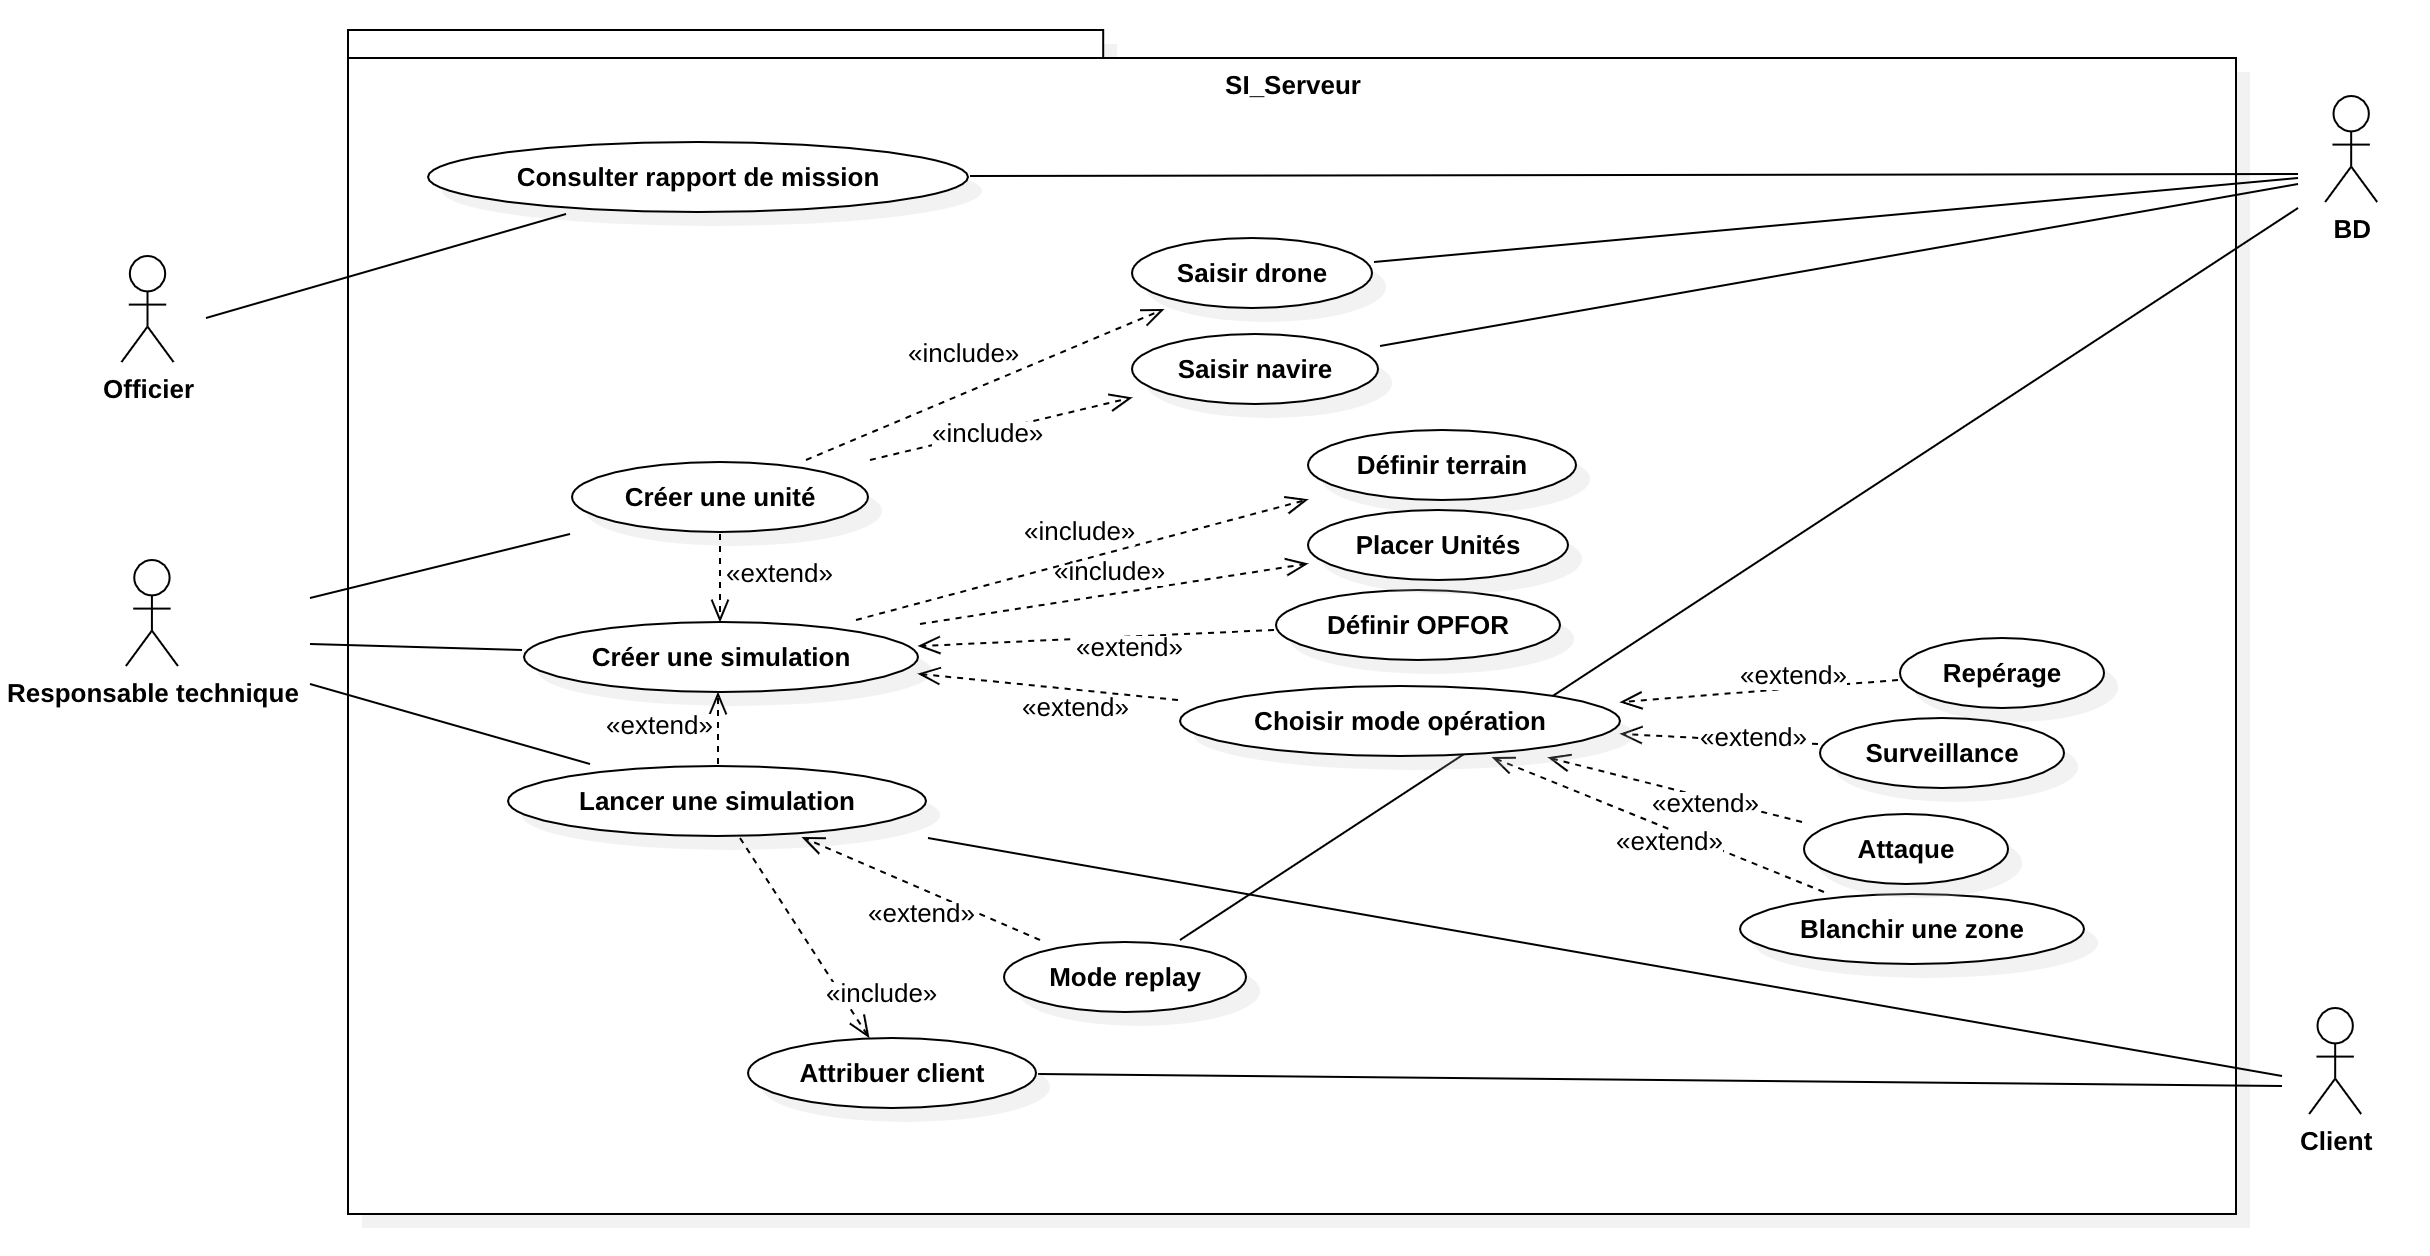
\includegraphics[height=8cm]{img/CUSI_Serveur.png} 
	\caption{CU SI Serveur.}
\end{figure}
\subsubsection{Diagramme de cas d'usage SI Client}
\begin{figure}[H]
	\centering
	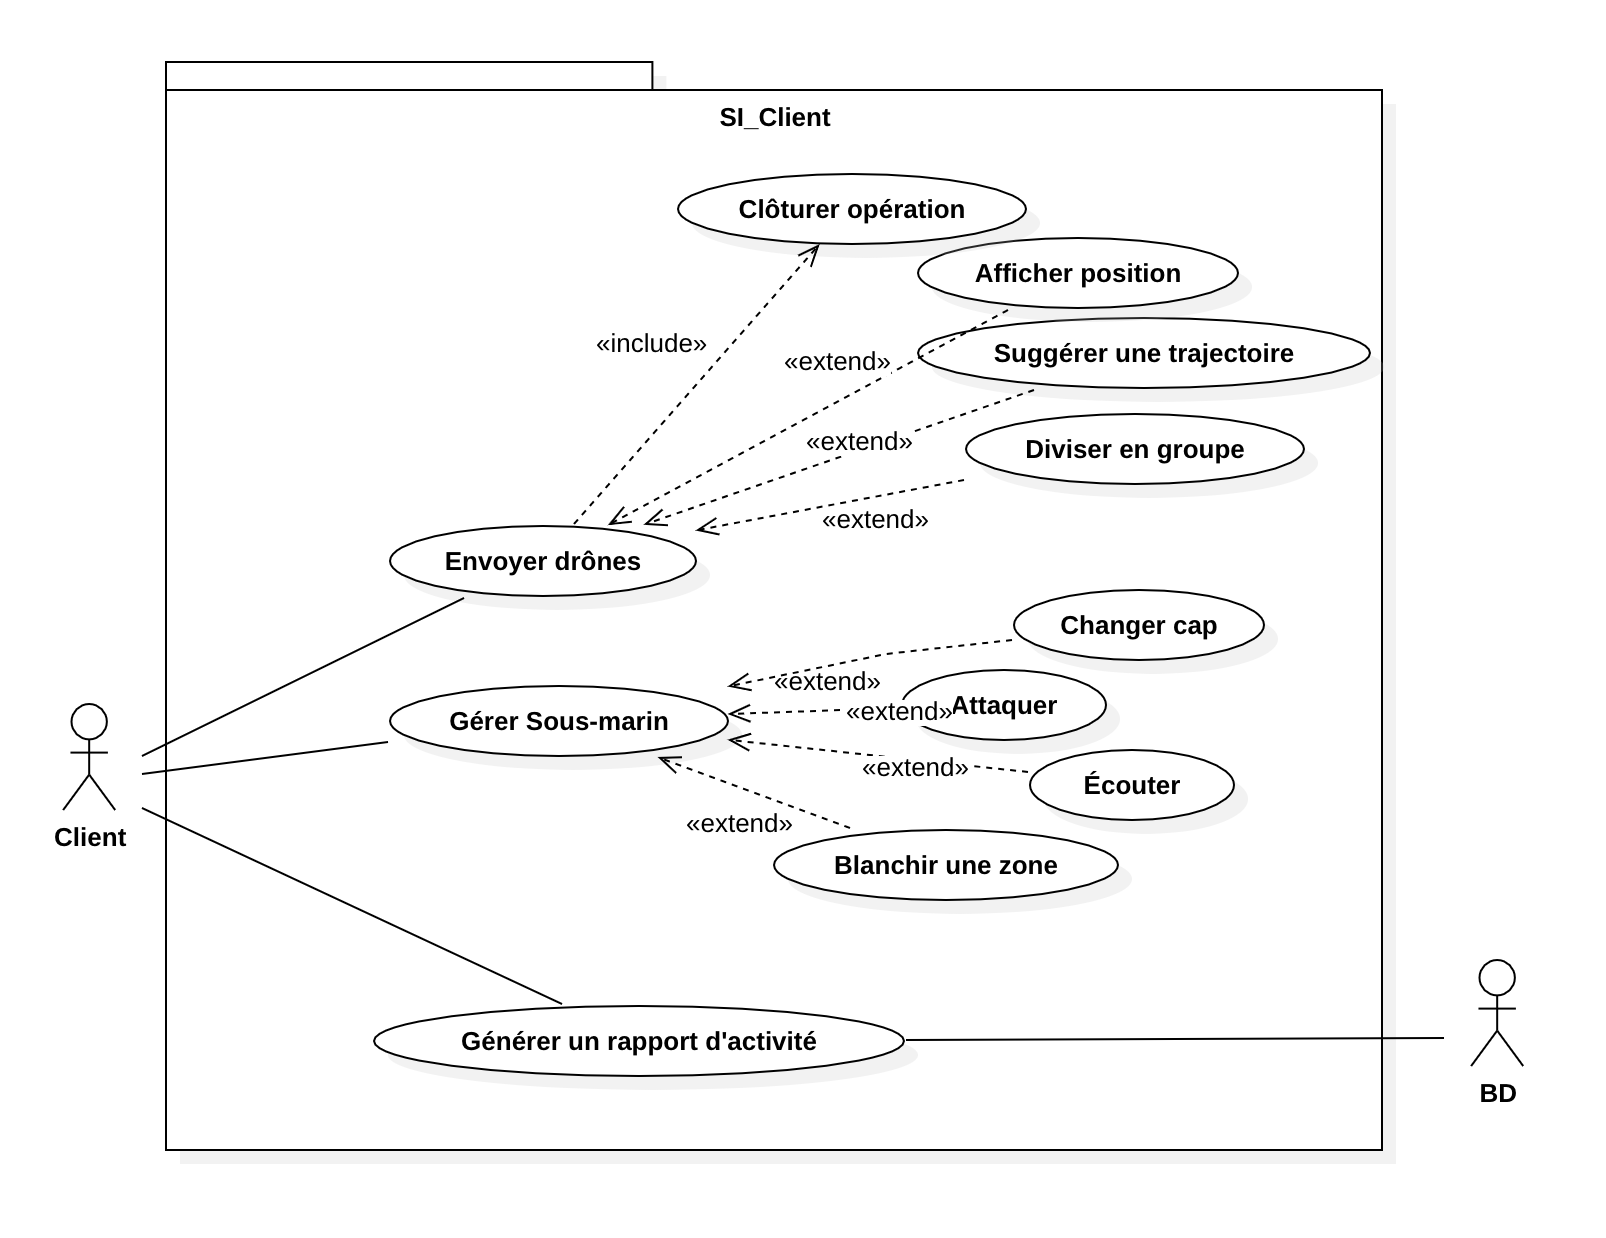
\includegraphics[height=13cm]{img/CUSI_Client.png} 
	\caption{CU SI Client.}
\end{figure}


\subsubsection{Structure du système niveau 1}
\begin{figure}[H]
	\centering
	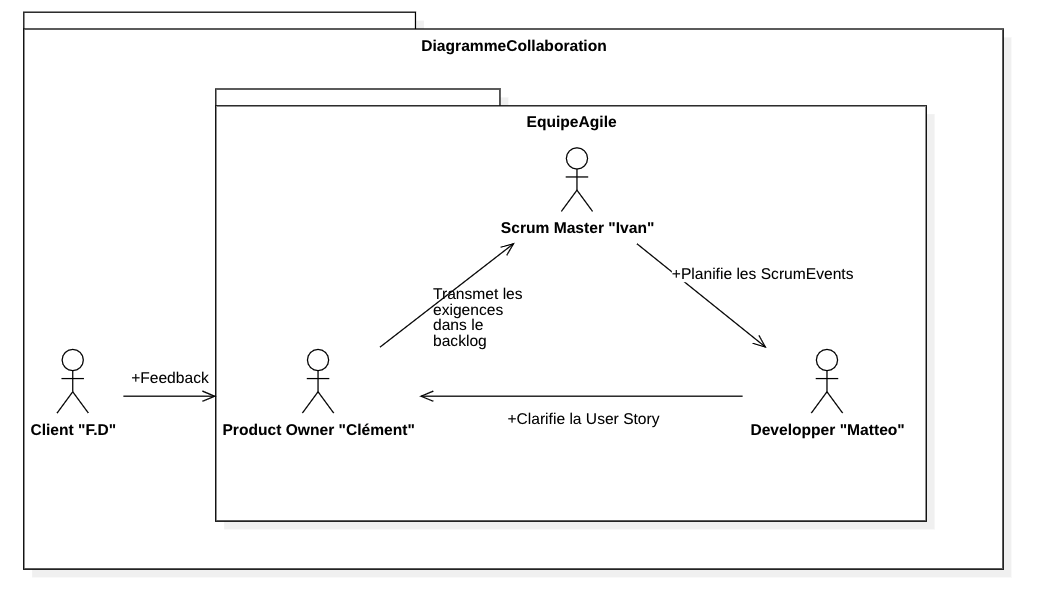
\includegraphics[height=8cm]{img/diagCollaboration.png} 
	\caption{Illustration de l'attribution des rôles principaux au sein de l'équipe.}
\end{figure}

\subsubsection{Structure du système niveau 2}
\begin{figure}[H]
	\centering
	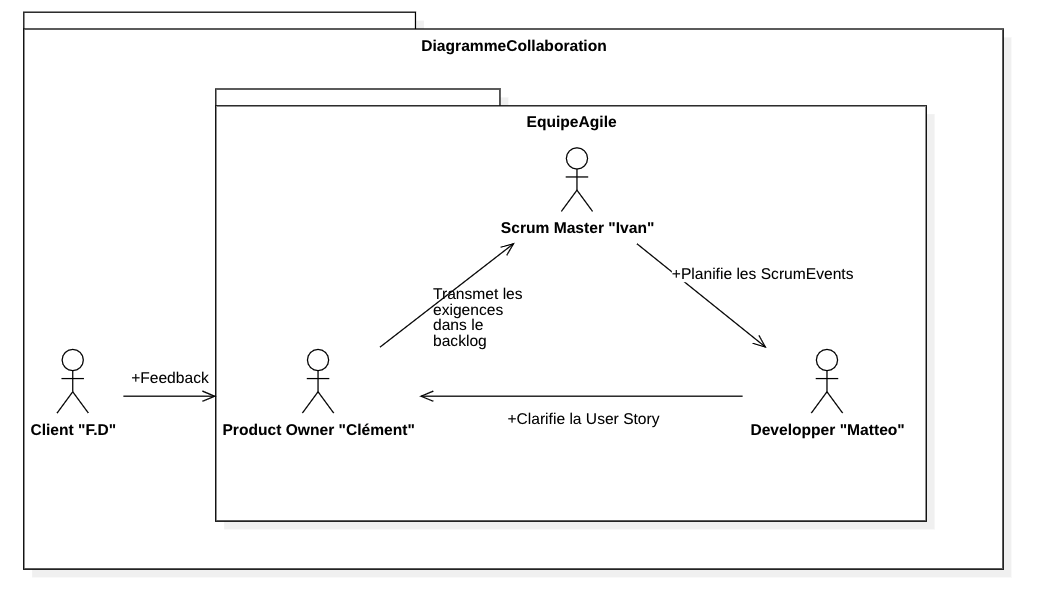
\includegraphics[height=8cm]{img/diagCollaboration.png} 
	\caption{Illustration de l'attribution des rôles principaux au sein de l'équipe.}
\end{figure}


\subsection{Axe statique}
\subsubsection{Diagramme des classes partie Serveur}
\begin{figure}[H]
	\centering
	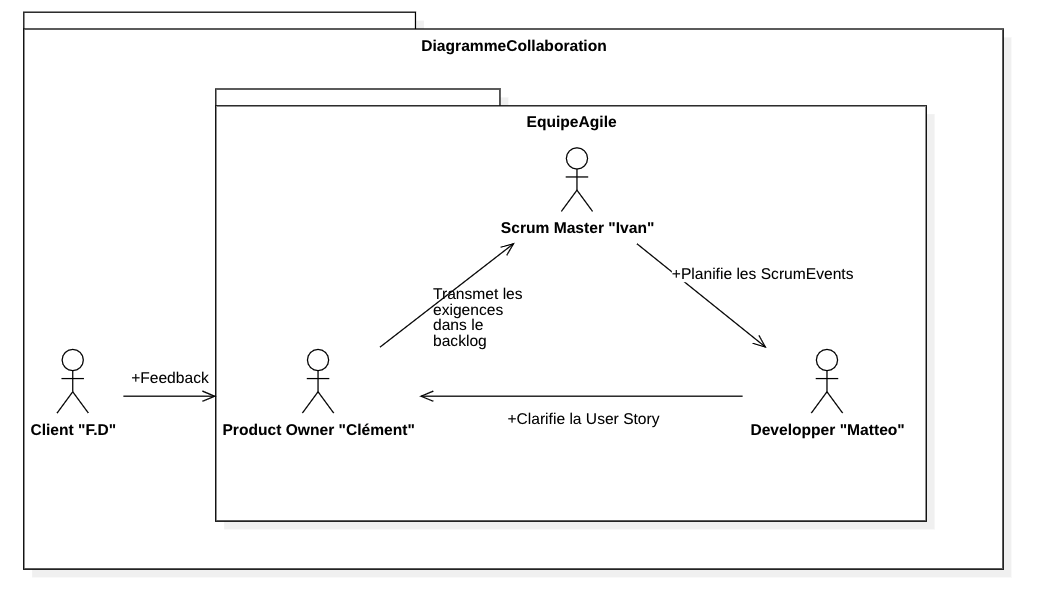
\includegraphics[height=8cm]{img/diagCollaboration.png} 
	\caption{Illustration de l'attribution des rôles principaux au sein de l'équipe.}
\end{figure}

\subsubsection{Diagramme des classes partie Client}
\begin{figure}[H]
	\centering
	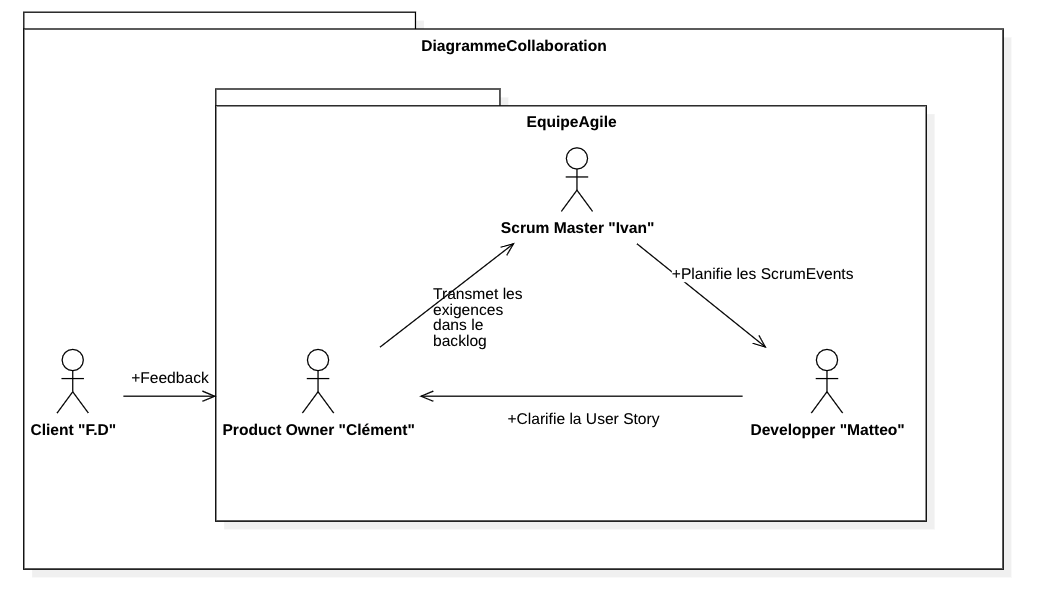
\includegraphics[height=8cm]{img/diagCollaboration.png} 
	\caption{Illustration de l'attribution des rôles principaux au sein de l'équipe.}
\end{figure}


\subsection{Axe dynamique}
\subsubsection{Diagramme de séquence Client-Serveur}
\begin{figure}[H]
	\centering
	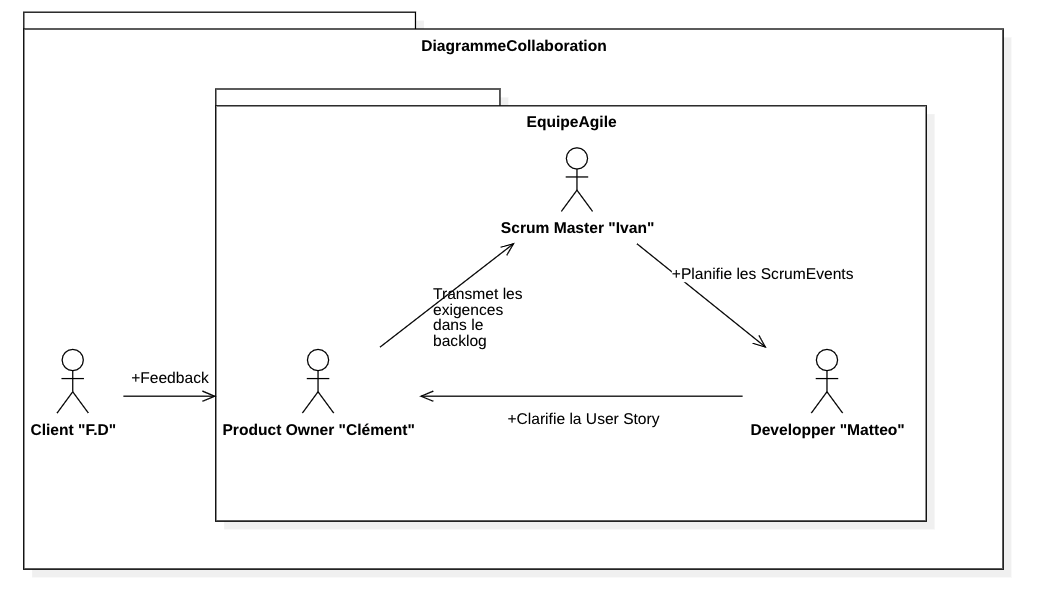
\includegraphics[height=8cm]{img/diagCollaboration.png} 
	\caption{Illustration de l'attribution des rôles principaux au sein de l'équipe.}
\end{figure}
